%iffalse
\let\negmedspace\undefined
\let\negthickspace\undefined
\documentclass[journal,12pt,onecolumn]{IEEEtran}
\usepackage{cite}
\usepackage{amsmath,amssymb,amsfonts,amsthm}
\usepackage{algorithmic}
\usepackage{graphicx}
\usepackage{textcomp}
\usepackage{xcolor}
\usepackage{txfonts}
\usepackage{listings}
\usepackage{enumitem}
\usepackage{mathtools}
\usepackage{gensymb}
\usepackage{comment}
\usepackage[breaklinks=true]{hyperref}
\usepackage{tkz-euclide} 
\usepackage{circuitikz}
\usepackage{listings}
\usepackage{gvv}      
%\def\inputGnumericTable{} 

\newcommand{\tripleprime}{{\prime\prime\prime}}



\usepackage{tikz}
\usepackage[latin1]{inputenc} 

\usepackage{caption}
\usepackage{subcaption}

\usepackage{color}                                            
\usepackage{array}                                            
\usepackage{longtable}                                       
\usepackage{calc}                                             
\usepackage{multirow}    
\usepackage{hhline}                                           
\usepackage{ifthen}     
\usepackage{tikz}
\usepackage{lscape}
\usepackage{tabularx}
\usepackage{array}
\usepackage{float}
\usepackage{multicol}
\usetikzlibrary{patterns}



\newtheorem{theorem}{Theorem}[section]
\newtheorem{problem}{Problem}
\newtheorem{proposition}{Proposition}[section]
\newtheorem{lemma}{Lemma}[section]
\newtheorem{corollary}[theorem]{Corollary}
\newtheorem{example}{Example}[section]
\newtheorem{definition}[problem]{Definition}
\newcommand{\BEQA}{\begin{eqnarray}}
\newcommand{\EEQA}{\end{eqnarray}}
\newcommand{\define}{\stackrel{\triangle}{=}}
\theoremstyle{remark}
\newtheorem{rem}{Remark}


\begin{document}
\bibliographystyle{IEEEtran}
\vspace{3cm}

\title{PH : GATE 2023}
\author{ai24btech11014 \\ Charitha Sri}

\maketitle
\bigskip       
\renewcommand{\thefigure}{\theenumi}
\renewcommand{\thetable}{\theenumi}

\section{27-39}
\begin{enumerate}

\item The $\Xi^{0^{*}}$ particle is a member of the Baryon decuplet with isospin state $|I, I_{3}\rangle = | \frac{1}{2}, \frac{1}{2} \rangle$ and strangeness quantum number $-2$. In the quark model, which one of the following is the flavour part of the $\Xi^{0^{*}}$ wavefunction?
\begin{enumerate}
\begin{multicols}{4}
\item $\frac{1}{\sqrt{2}}$\brak{ uss - ssu }
\item $\frac{1}{\sqrt{3}}$ \brak{uss + sus + ssu }
\item $\frac{1}{\sqrt{2}}$ \brak{ uss + ssu }
\item $\frac{1}{\sqrt{3}}$ \brak{ uss - sus + ssu }
\end{multicols}
\end{enumerate}

\item Which of the following is(are) the CORRECT option(s) for the Joule-Thomson effect?
\begin{enumerate}
\begin{multicols}{2}
\item It is an isentropic process
\item It is an isenthalpic process
\item It can result in cooling as well as heating
\item For an ideal gas, it always results in cooling
\end{multicols}
\end{enumerate}


\item The deuteron is a bound state of a neutron and a proton. Which of the following statements is (are) CORRECT?
\begin{enumerate}
\item The deuteron has a finite value of electric quadrupole moment due to non-spherical electronic charge distribution
\item The magnetic moment of the deuteron is equal to the sum of the magnetic moments of the neutron and the proton
\item The deuteron state is an admixture of $^{3}S_{1}$ and $^{3}D_{1}$ states
\item The deuteron state is an admixture of $^{3}S_{1}$ and $^{3}P_{1}$ states
\end{enumerate}


\item The Geiger-Muller counter is a device to detect $\alpha$, $\beta$, and $\gamma$ radiations. It is a cylindrical tube filled with monatomic gases like argon and polyatomic gases such as ethyl alcohol. The inner electrode is along the axis of the cylindrical tube, and the outer electrode is the tube. Which of the following statements is(are) CORRECT?
\begin{enumerate}
\item Argon is used so that ambient light coming from the surroundings does not produce any signal in the detector
\item Ethyl alcohol is used as a quenching gas
\item The electric field strength decreases from the axis to the edge of the tube and the direction of the field is radially outward
\item The electric field increases from the axis to the edge of the tube and the field direction is radially inward
\end{enumerate}


\item Consider an isolated magnetized sphere of radius $R$ with a uniform magnetization $\vec{M}$ along the positive $z$ direction, with the north and south poles of the sphere lying on the $z$ axis. It is given that the magnetic field inside the sphere is $\vec{B} = \frac{2\mu_{0}}{3}$ $\vec{M}$ where $\mu_{0}$ is thepermeability of vacuum. Which of the following statements is(are) CORRECT?

\begin{enumerate}
\item The bound volume current density is zero
\item The bound surface current density has maximum magnitude at the equator, where this magnitude equals $|\overrightarrow{M}|$
\item The auxiliary field $\vec{H} = -\frac{2}{3} \vec{M}$
\item Far from the sphere, the magnetic field is due to a dipole of moment $m$ , where $\frac{\vec{m}}{4\pi R^3} =\frac{B}{2\mu_{0}} \hat{z}$
\end{enumerate}


\item Which of the following options represent(s) linearly independent pair(s) of functions of a real variable $x$?

\begin{enumerate}
    \item $e^{ix}$ and $e^{-ix}$
    \item  $x$ and $e^{x}$
    \item $2^{x}$ and $2^{- 3 + x}$
    \item $e^{ix}$ and $\sin x$
\end{enumerate}

\item In the vector model of angular momentum applied to atoms, what is the minimum angle in degrees (in integer) made by the orbital angular momentum vector and the positive $z$ axis for a $2p$ electron?

\item For a transistor amplifier, the frequency response is such that the mid-band voltage gain is $200$. The cutoff frequencies are $20 Hz$ and $20 kHz$. What is the ratio (rounded off to two decimal places) of the voltage gain at $10 Hz$ to that at $100 kHz$?

\item An electric field as a function of radial coordinate $r$ has the form $\overrightarrow{E} = \alpha \frac{e^{-r^{2}}}{r} \hat{r}$, where $\alpha$ is a constant. Assume that dimensions are appropriately taken care of. The electric flux through a sphere of radius $\sqrt{2}$, centered at the origin, is $\Phi$. What is the value of $\frac{\Phi}{2\pi \alpha}$ (rounded off to two decimal places)?

\item It is given that the electronic ground state of a diatomic molecule $X_2$ has even parity and the nuclear spin of $X$ is $0$. Which one of the following is the CORRECT statement with regard to the rotational quantum number $J$ of this molecule?

\begin{enumerate}
    \item Lines of all $J$ values are present
    \item Lines have alternating intensity in the ratio of $3:1$
    \item Lines of only even $J$ values are present
    \item Lines of only odd $J$ values are present
\end{enumerate}


\item An input voltage in the form of a square wave of frequency $1 kHz$ is given to a circuit, which results in the output shown schematically below. Which one of the following options is the CORRECT representation of the circuit?


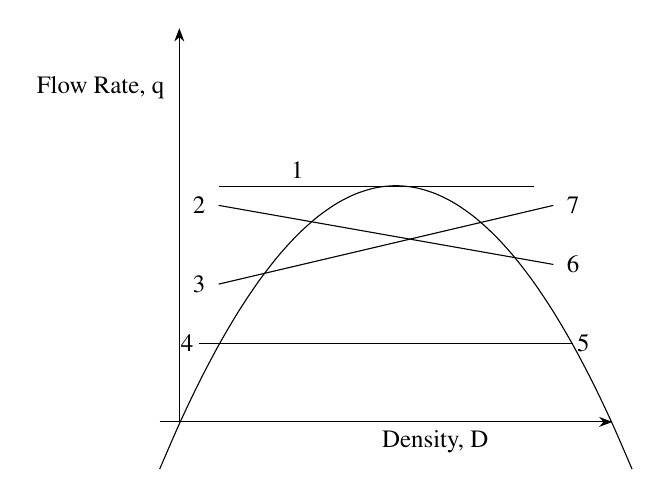
\begin{tikzpicture}

% Arrows for flow
\draw [->, >=Stealth] (6,9.5) -- (11.75,9.5);
\draw [->, >=Stealth] (6.25,9.5) -- (6.25,14.5);

% Labels for density and flow rate
\node [font=\small] at (9.5,9.25) {Density, D};
\node [font=\small] at (5.25,13.75) {Flow Rate, q};

% Short lines representing segments
\draw [-] (6.75,12.49) -- (10.75,12.49);
\draw [-] (6.75,11.25) -- (11,12.25);
\draw [-] (6.75,12.25) -- (11,11.5);
\draw [-] (6.5,10.5) -- (11.25,10.5);

% Labels for points
\node [font=\small] at (7.75,12.7) {1};
\node [font=\small] at (6.5,12.25) {2};
\node [font=\small] at (11.25,12.25) {7};
\node [font=\small] at (6.5,11.25) {3};
\node [font=\small] at (11.25,11.5) {6};
\node [font=\small] at (11.38,10.5) {5};
\node [font=\small] at (6.35,10.5) {4};

% Downward-opening parabola that passes through (6.5, 9.5) and (11.5, 9.5)
\draw[domain=6:12,smooth,variable=\x,black] plot (\x,{-(0.4*(\x - 9)^2) + 12.5}); 


\end{tikzpicture}


\begin{enumerate}
\item 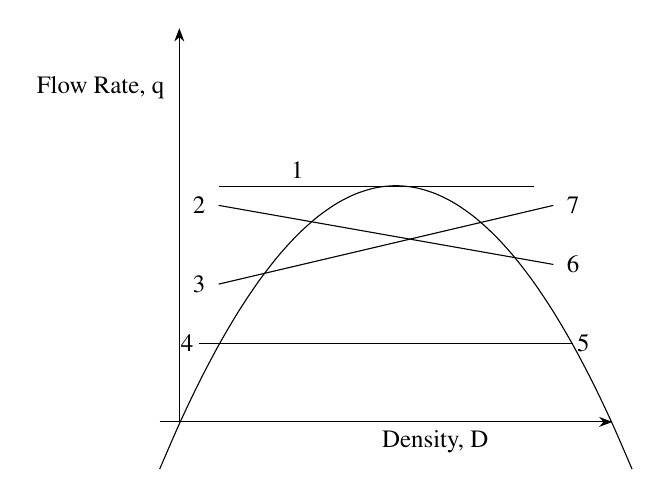
\begin{tikzpicture}

% Arrows for flow
\draw [->, >=Stealth] (6,9.5) -- (11.75,9.5);
\draw [->, >=Stealth] (6.25,9.5) -- (6.25,14.5);

% Labels for density and flow rate
\node [font=\small] at (9.5,9.25) {Density, D};
\node [font=\small] at (5.25,13.75) {Flow Rate, q};

% Short lines representing segments
\draw [-] (6.75,12.49) -- (10.75,12.49);
\draw [-] (6.75,11.25) -- (11,12.25);
\draw [-] (6.75,12.25) -- (11,11.5);
\draw [-] (6.5,10.5) -- (11.25,10.5);

% Labels for points
\node [font=\small] at (7.75,12.7) {1};
\node [font=\small] at (6.5,12.25) {2};
\node [font=\small] at (11.25,12.25) {7};
\node [font=\small] at (6.5,11.25) {3};
\node [font=\small] at (11.25,11.5) {6};
\node [font=\small] at (11.38,10.5) {5};
\node [font=\small] at (6.35,10.5) {4};

% Downward-opening parabola that passes through (6.5, 9.5) and (11.5, 9.5)
\draw[domain=6:12,smooth,variable=\x,black] plot (\x,{-(0.4*(\x - 9)^2) + 12.5}); 


\end{tikzpicture}

\item 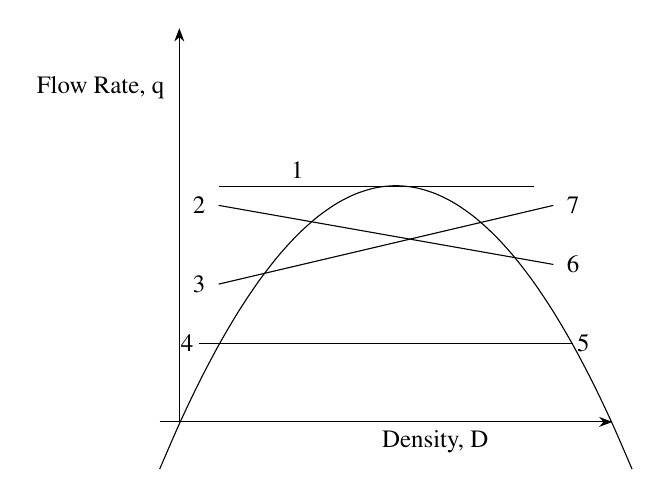
\begin{tikzpicture}

% Arrows for flow
\draw [->, >=Stealth] (6,9.5) -- (11.75,9.5);
\draw [->, >=Stealth] (6.25,9.5) -- (6.25,14.5);

% Labels for density and flow rate
\node [font=\small] at (9.5,9.25) {Density, D};
\node [font=\small] at (5.25,13.75) {Flow Rate, q};

% Short lines representing segments
\draw [-] (6.75,12.49) -- (10.75,12.49);
\draw [-] (6.75,11.25) -- (11,12.25);
\draw [-] (6.75,12.25) -- (11,11.5);
\draw [-] (6.5,10.5) -- (11.25,10.5);

% Labels for points
\node [font=\small] at (7.75,12.7) {1};
\node [font=\small] at (6.5,12.25) {2};
\node [font=\small] at (11.25,12.25) {7};
\node [font=\small] at (6.5,11.25) {3};
\node [font=\small] at (11.25,11.5) {6};
\node [font=\small] at (11.38,10.5) {5};
\node [font=\small] at (6.35,10.5) {4};

% Downward-opening parabola that passes through (6.5, 9.5) and (11.5, 9.5)
\draw[domain=6:12,smooth,variable=\x,black] plot (\x,{-(0.4*(\x - 9)^2) + 12.5}); 


\end{tikzpicture}

\item 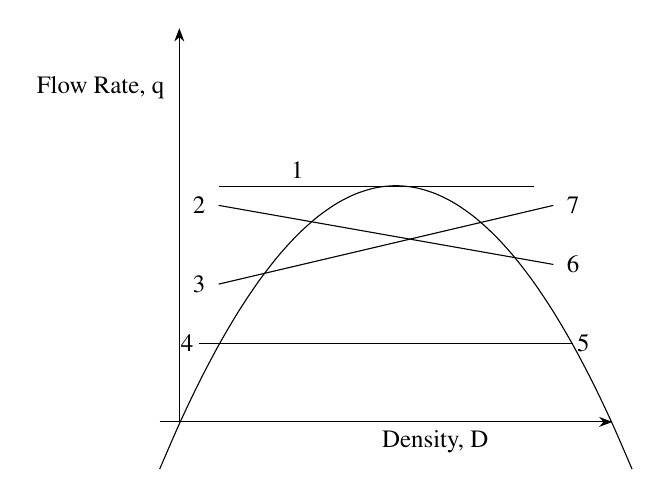
\begin{tikzpicture}

% Arrows for flow
\draw [->, >=Stealth] (6,9.5) -- (11.75,9.5);
\draw [->, >=Stealth] (6.25,9.5) -- (6.25,14.5);

% Labels for density and flow rate
\node [font=\small] at (9.5,9.25) {Density, D};
\node [font=\small] at (5.25,13.75) {Flow Rate, q};

% Short lines representing segments
\draw [-] (6.75,12.49) -- (10.75,12.49);
\draw [-] (6.75,11.25) -- (11,12.25);
\draw [-] (6.75,12.25) -- (11,11.5);
\draw [-] (6.5,10.5) -- (11.25,10.5);

% Labels for points
\node [font=\small] at (7.75,12.7) {1};
\node [font=\small] at (6.5,12.25) {2};
\node [font=\small] at (11.25,12.25) {7};
\node [font=\small] at (6.5,11.25) {3};
\node [font=\small] at (11.25,11.5) {6};
\node [font=\small] at (11.38,10.5) {5};
\node [font=\small] at (6.35,10.5) {4};

% Downward-opening parabola that passes through (6.5, 9.5) and (11.5, 9.5)
\draw[domain=6:12,smooth,variable=\x,black] plot (\x,{-(0.4*(\x - 9)^2) + 12.5}); 


\end{tikzpicture}

\item 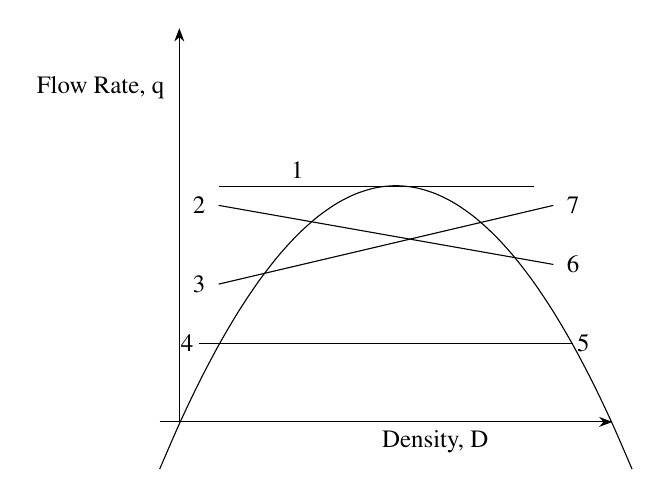
\begin{tikzpicture}

% Arrows for flow
\draw [->, >=Stealth] (6,9.5) -- (11.75,9.5);
\draw [->, >=Stealth] (6.25,9.5) -- (6.25,14.5);

% Labels for density and flow rate
\node [font=\small] at (9.5,9.25) {Density, D};
\node [font=\small] at (5.25,13.75) {Flow Rate, q};

% Short lines representing segments
\draw [-] (6.75,12.49) -- (10.75,12.49);
\draw [-] (6.75,11.25) -- (11,12.25);
\draw [-] (6.75,12.25) -- (11,11.5);
\draw [-] (6.5,10.5) -- (11.25,10.5);

% Labels for points
\node [font=\small] at (7.75,12.7) {1};
\node [font=\small] at (6.5,12.25) {2};
\node [font=\small] at (11.25,12.25) {7};
\node [font=\small] at (6.5,11.25) {3};
\node [font=\small] at (11.25,11.5) {6};
\node [font=\small] at (11.38,10.5) {5};
\node [font=\small] at (6.35,10.5) {4};

% Downward-opening parabola that passes through (6.5, 9.5) and (11.5, 9.5)
\draw[domain=6:12,smooth,variable=\x,black] plot (\x,{-(0.4*(\x - 9)^2) + 12.5}); 


\end{tikzpicture}

\end{enumerate}

\item A simple harmonic oscillator with an angular frequency $\omega$ is in thermal equilibrium with a reservoir at absolute temperature $T$, with $\omega = \frac{2 k_{B} T}{\hbar}$. Which one of the following is the partition function $Z$ of the system?
\begin{enumerate}
\item $\frac{e}{e^{2} - 1}$
\item $\frac{e}{e^{2}  + 1}$
\item $\frac{e}{e - 1}$
\item $\frac{e}{e + 1}$
\end{enumerate}

\item Which one of the following options is the most appropriate match between the items given in Column 1 and Column 2?

\begin{table}[h]
        \centering
        \begin{tabular}{ c@{\hskip 1cm }c }
            Group I & Group II \\
            P. Alidade & 1. Chain surveying \\
            Q. Arrow & 2. Levelling \\
            R. Bubble tube & 3. Plain table surveying \\
            S. Stadia hair & 4. Theodolite surveying \\
        \end{tabular}
    \end{table}


\begin{enumerate}
    \item (i) T; (ii) P,S,T; (iii) Q,R; (iv) S
    \item (i) P, T; (ii) S; (iii) R, S; (iv) S, T
    \item (i) T; (ii) R, S; (iii) Q, R; (iv) S
    \item (i) S, T; (ii) P, S; (iii) R, T; (iv) S
\end{enumerate}


\end{enumerate}
\end{document}
